\documentclass[11pt]{article}

\usepackage{amsmath}
\usepackage{amsfonts} 
\usepackage{amsthm}
\usepackage{enumitem} 
\usepackage{mathtools}
\usepackage{tikz}
\usepackage[top=2cm,bottom=2cm,left=2cm,right=2cm,marginparwidth=1.75cm]{geometry}
\setlength{\parindent}{0cm}

\newcommand{\R}{\mathbb{R}}
\newcommand\simpleGraph[1]{
  \begin{tikzpicture}[every node/.style={circle,draw}]
    \node (a) at (0,1) {};
    \node (b) at (1,1) {};
    \node (c) at (1,0) {};
    \node (d) at (0,0) {};

    \foreach \from/\to in {#1}
      \draw (\from) -- (\to);
  \end{tikzpicture}\hfil
}
\newcommand\itm[1]{\item[\textbf{#1}]}

\pagenumbering{gobble}
\newtheorem{theorem}{Theorem}

\title{\vspace{-1.0cm}MATH 5707 Homework 1}
\author{Fletcher Gornick}
\date{January 18, 2022}

\begin{document}
\maketitle
\begin{itemize}
  \itm{1.2.4} Show that there are eleven nonisomorphic simple graphs on four vertices.

    \simpleGraph{}
    \simpleGraph{a/b}
    \simpleGraph{a/b,a/d}
    \simpleGraph{a/d,b/c}
    \simpleGraph{a/b,a/c,a/d}
    \simpleGraph{a/d,a/b,b/c}

    \simpleGraph{a/b,a/d,b/d}
    \simpleGraph{a/b,b/c,c/d,d/a}
    \simpleGraph{a/b,b/d,c/d,d/a}
    \simpleGraph{a/b,b/c,c/d,d/a,a/c}
    \simpleGraph{a/b,b/c,c/d,d/a,a/c,b/d}

  \itm{1.2.10} The \textit{\(k\)-cube} is the graph whose vertices are the ordered \(k\)-tuples of 0's and 1's, two vertices being joined if and only if they differ in exactly one coordinate.  Show that the \(k\)-cube has \(2^k\) vertices, \(k 2^{k-1}\) edges and is bipartite.

  \itm{1.2.11} \begin{enumerate}[label=(\alph*)]
      \item The \textit{complement} \(G^c\) of a simple graph \(G\) is the simple graph with vertex set \(V\), two vertices being adjacent in \(G^c\) if and only if they are not adjacent in \(G\). Describe the graphs \(K^c_n\) and \(K^c_{m,n}\).
      \item A simple graph \(G\) is \textit{self-complementary} if \(G \cong G^c\). Show that if \(G\) is self-complementary, then \(v \equiv 0,1 \pmod 4\)
    \end{enumerate}

  \itm{1.4.4} Find a bipartite graph that is not isomorphic to a subgraph of any \(k\)-cube.

  \itm{1.5.5} If \(G\) has vertices \(v_1, v_2, \hdots, v_v\), the sequence \((d(v_1), d(v_2), \hdots, d(v_v))\) is called a \textit{degree sequence} of \(G\).  Show that a sequence (\(d_1, d_2, \hdots, d_n\)) of non-negative integers is a degree sequence of some graph if and only if \(\displaystyle \sum_{i=1}^n d_i\) is even.

  \itm{1.5.7(a)} Let \(\textbf{d} = (d_1, d_2, \hdots, d_n)\) be a nonincreasing sequence of non-negative integers, and denote the sequence \((d_2-1, d_3-1, \hdots, d_{d_1+1}-1, d_{d_1+2}-1, \hdots, d_n)\) by \(\textbf{d'}\).  Show that \(\textbf{d}\) is graphic if and only if \(\textbf{d'}\) is graphic.

  \itm{1.5.10} The \textit{edge graph} of a graph \(G\) is the graph with vertex set \(E(G)\) in which two vertices are joined if and only if they are adjacent edges in \(G\).  Show that, if \(G\) is simple
    \begin{enumerate}[label=(\alph*)]
      \item the edge graph of \(G\) has \(\varepsilon(G)\) vertices and \(\displaystyle\sum_{v \in V(G)} \begin{pmatrix} d_G(v) \\ 2 \end{pmatrix}\) edges;
      \item the edge graph of \(K_5\) is isomorphic to the complement of the graph featured in exercise 1.2.6.
    \end{enumerate}

  \itm{1.6.7} Show that if \(G\) is disconnected, then \(G^c\) is connected.

  \itm{1.6.10} Show that any two longest paths in a connected graph have a vertex in common.

  \itm{1.7.2} Show that if \(\delta \geq 2\), then \(G\) contains a cycle.

  \itm{1.7.3} Show that if \(G\) is simple and \(\delta \geq 2\), then \(G\) contains a cycle of length at least \(\delta + 1\).

  \itm{4.1.1} Which of the following figures can be drawn without lifting one's pen from the paper or covering a line more than once?

    \resizebox{0.25\textwidth}{4cm}{
      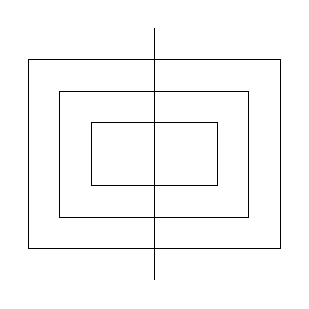
\begin{tikzpicture}[scale=0.4]
        \draw (4,0) -- (4,8);
        \draw (0,1) rectangle (8,7);
        \draw (1,2) rectangle (7,6);
        \draw (2,3) rectangle (6,5);
      \end{tikzpicture}
    }\hfil
    \resizebox{0.25\textwidth}{4cm}{
      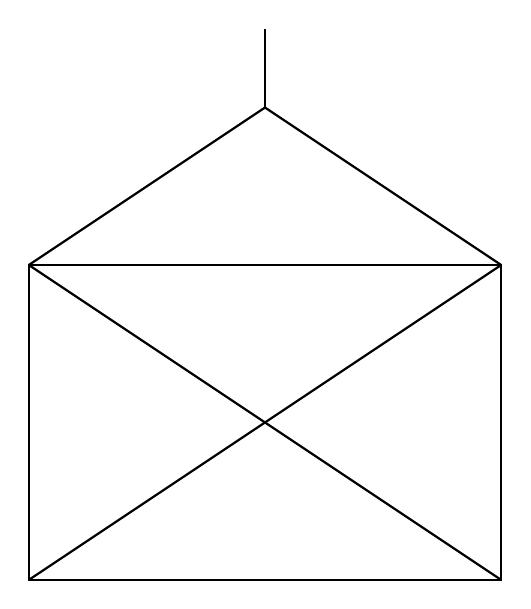
\begin{tikzpicture}
        \draw[thick] (0,0) rectangle (6,4);
        \draw[thick] (0,0) -- (6,4);
        \draw[thick] (0,4) -- (6,0);
        \draw[thick] (0,4) -- (3,6);
        \draw[thick] (6,4) -- (3,6);
        \draw[thick] (3,6) -- (3,7);
      \end{tikzpicture}
    }\hfil
    \resizebox{0.25\textwidth}{4cm}{
      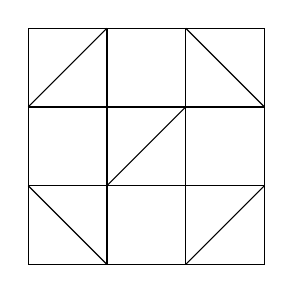
\begin{tikzpicture}
        \draw (0,0) rectangle (3,3);
        \draw (0,1) -- (3,1);
        \draw (0,2) -- (3,2);
        \draw (1,0) -- (1,3);
        \draw (2,0) -- (2,3);
        \draw (0,2) -- (1,3);
        \draw (2,3) -- (3,2);
        \draw (0,1) -- (1,0);
        \draw (2,0) -- (3,1);
        \draw (1,1) -- (2,2);
      \end{tikzpicture}
    }

  \itm{4.1.2} If possible, draw an eulerian graph \(G\) with \(v\) even and \(\varepsilon\) odd; otherwise, explain why there is no such graph.

  \itm{4.2.2} A mouse eats his way through a \(3 \times 3 \times 3\) cube of cheese by tunnelling through all of the 27 \(1 \times 1 \times 1\) subcubes.  If he starts at one corner and always moves on to an uneaten subcube, can he finish at the centre of the cube?

  \itm{4.2.3} Show that if \(G\) has a Hamilton path then, for every proper subset \(S\) of \(V\), \(\omega(G-S) \leq |S|+1\).

\end{itemize}
\end{document}
